\section{Szczegóły implementacyjne -- AES}
\label{sec:szczegoly-implementacyjne-aes}
Szyfrowanie i deszyfrowanie jest realizowane w sposób zgodny ze standardem AES \cite{aes-standard}. Moduły szyfrujący i deszyfrujący działają w sposób asynchroniczny -- nie są taktowane zegarem. Takie rozwiązanie zostało wybrane ze względu na fakt, że wąskim gardłem systemu jest kanał komunikacji. Próby poprawy wydajności szyfrowania oraz deszyfrowania np. poprzez implementację przetwarzania potokowego (ang. \textit{pipelining}) nie przyniosłyby skutku ze względu na bardzo niską osiągalną prędkość transmisji (rozdz. \ref{sec:uart-parametry}).

Logika AES jest zaimplementowane w języku VHDL jako funkcje, które zostały zdekomponowane do niewielkich składowych w celu poprawy czytelności kodu.

\subsection{Arytmetyka w ciele \textit{GF($2^8$)}}
\label{sec:arytmetyka}
Transformacje stanu używane przez Algorytm AES są zdefiniowane przy pomocy działań na wielomianach o współczynnikach należących do ciała skończonego \textit{GF($2^8$)} \cite[rozdz. 4.3]{aes-standard}. Arytmetyka w tym ciele różni się od arytmetyki w ciele liczb rzeczywistych.

\paragraph{Dodawanie w ciele \textit{GF($2^8$)}} \cite[rozdz. 4.1]{aes-standard} jest operacją XOR. Takie działanie jest dostępne w języku VHDL, więc nie wymagało implementacji specjalnej procedury.

\paragraph{Mnożenie w ciele \textit{GF($2^8$)}} \cite[rozdz. 4.2]{aes-standard} jest równoważne mnożeniu wielomianów modulo pewien wielomian nierozkładalny -- dla AES jest to wielomian
\begin{equation*}
m(x) = x^8 + x^4 + x^3 + x + 1
\end{equation*}
To działanie jest zaimplementowane jako funkcja \textit{multiply}(listing \ref{lst:multiply-impl}) realizująca zmodyfikowany algorytm dodawania \textit{peasant's algorithm} \cite{multiply-algo}.

\begin{figure}[!h]
\begin{lstlisting}[style=vhdl, captionpos=b, caption={Mnożenie wielomianów w ciele \textit{GF($2^8$)}}, label={lst:multiply-impl}]
function multiply (left  : std_logic_vector(7 downto 0); 
                   right : std_logic_vector(7 downto 0)) 
return std_logic_vector is
	
constant irred_poly      : std_logic_vector(7 downto 0) := x"1b";
variable a               : std_logic_vector(7 downto 0) := (others => '0');
variable b               : std_logic_vector(7 downto 0) := (others => '0');
variable p               : std_logic_vector(7 downto 0) := (others => '0');
variable extended_b_lsb  : std_logic_vector(7 downto 0) := (others => '0');
variable extended_a_carry: std_logic_vector(7 downto 0) := (others => '0');

begin
	a := left;
	b := right;
	p := (others => '0');

	for i in 0 to 7 loop
		--1
		extended_b_lsb := (others => b(0));
		p := p xor (extended_b_lsb and a);

		--2
		b := '0' & b(7 downto 1);

		--3
		extended_a_carry := (others => a(7));

		--4
		a := a(6 downto 0) & '0';

		--5
		a := a xor (extended_a_carry and irred_poly);
	end loop;
		
	return p;
end function;
\end{lstlisting}
\end{figure}


\newpage
\subsection{Transformacje stanu}
Algorytm AES przy szyfrowaniu oraz rozwinięciu klucza wykorzystuje cztery podstawowe transformacje stanu.

\paragraph{SubBytes} \cite[rozdz. 5.1.1]{aes-standard} jest transformacją realizującą nieliniowe podstawienie bajtów. Każdy bajt stanu jest zastąpiony odpowiadającym mu bajtem \cite[rys. 6]{aes-standard} z tablicy podstawień S-Box \cite[rys. 7]{aes-standard}, która jest zaimplementowana jako tablica predefiniowanych stałych (listing. \ref{lst:s-box}). Pobranie z tablicy wartości do podstawienia realizowane jest przez funkcję \textit{lookup\_sub}. Transformacja SubBytes jest funkcją korzystającą ze zdefiniowanego S-Box (listing \ref{lst:sub-bytes}).

\paragraph{ShiftRows} \cite[rozdz. 5.1.2]{aes-standard} jest transformacją polegającą na cyklicznym przesunięciu trzech ostatnich rzędów stanu w lewo odpowiednio o 1, 2 lub 3 pozycje \cite[rys. 8]{aes-standard} (listing \ref{lst:shift-rows}).

\paragraph{AddRoundKey} \cite[rozdz. 5.1.3]{aes-standard} jest transformacją polegającą na dodaniu (operacja XOR, rozdz. \ref{sec:arytmetyka}) do stanu klucza rundy \cite[rys. 10]{aes-standard} (listing \ref{lst:add-round-key}). Wszystkie rundy posiadają oddzielne klucze, które są wygenerowane przy pomocy procedury rozwinięcia klucza (rozdz. \ref{sec:key-expansion}).

\paragraph{MixColumns} \cite[rozdz. 5.1.3]{aes-standard} jest transformacją operującą na kolumnach, która taktuje je jako wielomiany o współczynnikach należących do ciała \textit{GF($2^8$)}, będących wartościami odpowiednich bajtów stanu. Każda z kolumn jest pomnożona modulo $x^4 + 1$ przez wielomian $a(x)$ \cite[rys. 9]{aes-standard}.
\begin{equation*}
a(x) = 3x^3 + x^2 + x + 2
\end{equation*}
Transformacja MixColumns jest zaimplementowana jako funkcja modyfikująca stan według wzorów wyprowadzonych w dokumencie stanowiącym standard AES \cite[rozdz. 5.1.3]{aes-standard} (listing \ref{lst:mix-columns}).


\begin{figure}[!h]
\begin{lstlisting}[style=vhdl, captionpos=b, caption={Implementacja S-Box}, label={lst:s-box}]
type t_sub_table is array (0 to 255) of std_logic_vector(7 downto 0);

constant sub_table : t_sub_table := (
	------|   0      1      2      3      4      5     ...     e      f
	------|------|------|------|------|------|------|------|------|------|
	/* 0 */ x"63", x"7c", x"77", x"7b", x"f2", x"6b",  ... , x"ab", x"76",
	/* 1 */ x"ca", x"82", x"c9", x"7d", x"fa", x"59",  ... , x"72", x"c0",
	/* 2 */ x"b7", x"fd", x"93", x"26", x"36", x"3f",  ... , x"31", x"15",
	/* 3 */ x"04", x"c7", x"23", x"c3", x"18", x"96",  ... , x"b2", x"75",
	/* 4 */ x"09", x"83", x"2c", x"1a", x"1b", x"6e",  ... , x"2f", x"84",
	/* 5 */ x"53", x"d1", x"00", x"ed", x"20", x"fc",  ... , x"58", x"cf",
	/* 6 */ x"d0", x"ef", x"aa", x"fb", x"43", x"4d",  ... , x"9f", x"a8",
	/* 7 */ x"51", x"a3", x"40", x"8f", x"92", x"9d",  ... , x"f3", x"d2",
	/* 8 */ x"cd", x"0c", x"13", x"ec", x"5f", x"97",  ... , x"19", x"73",
	/* 9 */ x"60", x"81", x"4f", x"dc", x"22", x"2a",  ... , x"0b", x"db",
	/* a */ x"e0", x"32", x"3a", x"0a", x"49", x"06",  ... , x"e4", x"79",
	/* b */ x"e7", x"c8", x"37", x"6d", x"8d", x"d5",  ... , x"ae", x"08",
	/* c */ x"ba", x"78", x"25", x"2e", x"1c", x"a6",  ... , x"8b", x"8a",
	/* d */ x"70", x"3e", x"b5", x"66", x"48", x"03",  ... , x"1d", x"9e",
	/* e */ x"e1", x"f8", x"98", x"11", x"69", x"d9",  ... , x"28", x"df",
	/* f */ x"8c", x"a1", x"89", x"0d", x"bf", x"e6",  ... , x"bb", x"16");

function lookup_sub (index : std_logic_vector(7 downto 0)) 
return std_logic_vector is begin
	return sub_table(to_integer(unsigned(index)));
end function;
\end{lstlisting}
\end{figure}

\begin{figure}[!p]
\begin{lstlisting}[style=vhdl, captionpos=b, caption={Implementacja transformacji stanu SubBytes}, label={lst:sub-bytes}]
function sub_bytes (state_in : aes_state) return aes_state is 
	variable state_out : aes_state;
begin
	for r in 0 to 3 loop
		for c in 0 to 3 loop
			state_out(r, c) := lookup_sub(state_in(r, c));
		end loop;
	end loop;
		
	return state_out;
end function;
\end{lstlisting}
\end{figure}


\begin{figure}[!p]
\begin{lstlisting}[style=vhdl, captionpos=b, caption={Implementacja transformacji stanu ShiftRows}, label={lst:shift-rows}]
function shift_rows (state_in : aes_state) return aes_state is
 	variable state_out : aes_state;
begin
	for r in 0 to 3 loop
		for c in 0 to 3 loop
			state_out(r, c) := state_in(r, (c + r) mod 4);
		end loop;
	end loop;
		
	return state_out;
end function;
\end{lstlisting}
\end{figure}


\begin{figure}[!p]
\begin{lstlisting}[style=vhdl, captionpos=b, caption={Implementacja transformacji stanu AddRoundKey}, label={lst:add-round-key}]
function add_round_key state_in      : aes_state; 
                       key_expansion : std_logic_vector; 
                       round_number  : Integer) return aes_state is
	constant byte_bits   : Integer := 8;
	constant word_length : Integer := 4 * 8;
	constant Nb          : Integer := 4;

	variable key_word    : std_logic_vector(word_length - 1 downto 0);
 	variable state_out   : aes_state;
begin
	for c in 0 to 3 loop
		key_word := key_expansion((round_number * Nb + 1 + c) * word_length-1 
			downto (round_number * Nb + c) * word_length);
		for r in 0 to 3 loop
			state_out(r, c) := state_in(r, c) 
				xor key_word(byte_bits * (r + 1) - 1 downto byte_bits * r);
		end loop;
	end loop;

	return state_out;
end function;
\end{lstlisting}
\end{figure}

\begin{figure}[!t]
\begin{lstlisting}[style=vhdl, captionpos=b, caption={Implementacja transformacji stanu MixColumns}, label={lst:mix-columns}]
function mix_columns  state_in : aes_state) return aes_state is
	variable state_out : aes_state;
begin
	for c in 0 to 3 loop
		state_out(0, c) :=     multiply(x"02", state_in(0, c)) 
		                   xor multiply(x"03", state_in(1, c))
		                   xor                 state_in(2, c)  
		                   xor                 state_in(3, c);
				
		state_out(1, c) :=                     state_in(0, c)  
		                   xor multiply(x"02", state_in(1, c)) 
		                   xor multiply(x"03", state_in(2, c)) 
		                   xor                 state_in(3, c);
				
		state_out(2, c) :=                     state_in(0, c)  
		                   xor                 state_in(1, c)
		                   xor multiply(x"02", state_in(2, c)) 
		                   xor multiply(x"03", state_in(3, c));
		   			
		state_out(3, c) :=     multiply(x"03", state_in(0, c)) 
		                   xor                 state_in(1, c)
		                   xor                 state_in(2, c)  
		                   xor multiply(x"02", state_in(3, c));
	end loop;

	return state_out;
end;
\end{lstlisting}
\end{figure}

\newpage
\subsection{Rozwinięcie klucza}
\label{sec:key-expansion}
Algorytm AES w każdej rundzie potrzebuje osobnego 128-bitowego klucza rundy. Aby otrzymać te klucze rozwija się 256-bitowy klucz szyfrowania przy pomocy algorytmu Rijndael'a (ang. \textit{Rijndael key schedule}) \cite[rozdz. 5.2]{aes-standard}. Procedura została zaimplementowana jako funkcja (listing \ref{lst:key-schedule}) działająca według algorytmu opisanego w standardzie AES \cite[rys. 11]{aes-standard}.

\begin{figure}[!p]
\begin{lstlisting}[style=vhdl, captionpos=b, caption={Implementacja rozwinięcia klucza -- \textit{Rijndael key schedule}}, label={lst:key-schedule}]
function key_expansion256 (key : std_logic_vector) 
return std_logic_vector is

constant word_length : Integer := 4 * 8;
constant byte_bits   : Integer := 8;
constant Nk          : Integer := 8;
	
variable tmp         : std_logic_vector(word_length - 1 downto 0);
variable tmp2        : std_logic_vector(word_length - 1 downto 0);
variable rcon        : std_logic_vector(word_length - 1 downto 0);
variable result      : std_logic_vector(60 * word_length - 1 downto 0);

begin

result(word_length * Nk - 1 downto 0) := key;
for i in Nk to 59 loop
	tmp := result(word_length * i - 1 downto word_length * (i - 1));
	
	if (i mod Nk = 0) then
		--RotWord
		tmp2 := tmp;
		tmp(word_length - 1 downto word_length - byte_bits) := 
			tmp2(byte_bits - 1 downto 0);
		tmp(word_length - byte_bits - 1 downto 0) := 
			tmp2(word_length - 1 downto byte_bits);

		--SubWord
		for j in 0 to 3 loop
			tmp((j + 1) * byte_bits - 1 downto j * byte_bits) := 
				lookup_sub(tmp((j + 1) * byte_bits - 1 downto j * byte_bits));
		end loop;

		--Rcon XOR
		tmp(byte_bits - 1 downto 0) := 
			tmp(byte_bits - 1 downto 0) 
			  xor std_logic_vector(to_unsigned(2 ** (i / Nk - 1), byte_bits));

	elsif (i mod Nk = 4) then
		--SubWord
		for j in 0 to 3 loop
			tmp((j + 1) * byte_bits - 1 downto j * byte_bits) := 
				lookup_sub(tmp((j + 1) * byte_bits - 1 downto j * byte_bits));
		end loop;
	end if;
	
	result(word_length * (i + 1) - 1 downto word_length * i) := 
		tmp xor result(word_length * (i-Nk+1)-1 downto word_length * (i-Nk));
end loop;
return result;

end function;
\end{lstlisting}
\end{figure}

\newpage
\subsection{Moduł szyfrujący AES}
Logika szyfrująca została zaimplementowana jako funkcja realizująca algorytm opisany w standardzie AES \cite[rozdz. 5.1, rys. 5]{aes-standard} (listing \ref{lst:aes-encryption}). Korzysta ona ze zdefiniowanych funkcji pomocniczych wykonujących kolejne rundy przekształcenia (listing \ref{lst:rounds}).

Moduł szyfrujący AES przyjmuje rozwinięcie klucza i blok tekstu jawnego oraz zwraca tekst zaszyfrowany. Jest zaimplementowany jako wywołanie funkcji szyfrującej (listing. \ref{lst:aes-encryption-module}).

Opis sygnałów interfejsu modułu \textit{aes256enc}:
\begin{interface}{KEY\_EXPANSION}
	\item[\insignal{KEY\_EXPANSION}] rozwinięcie klucza AES.
	\item[\insignal{PLAINTEXT}] blok tekstu jawnego.
	\item[\outsignal{CYPHERTEXT}] blok tekstu zaszyfrowanego.
\end{interface}

\begin{figure}[!h]
\begin{lstlisting}[style=vhdl, captionpos=b, caption={Implementacja funkcji szyfrującej AES}, label={lst:aes-encryption}]
function encode256 (plaintext     : std_logic_vector; 
                    key_expansion : std_logic_vector) 
return std_logic_vector is
	variable cyphertext    : std_logic_vector(127 downto 0);
	variable state         : aes_state;
	begin
	for r in 0 to 3 loop
		for c in 0 to 3 loop
			state(r, c) := plaintext((r + 4 * c + 1) * 8-1 downto (r+4*c)*8);
		end loop;
	end loop;

	state := round_0(state, key_expansion);

	for i in 1 to 13 loop
		state := round_n(state, key_expansion, i);
	end loop;

	state := round_last(state, key_expansion);

	for r in 0 to 3 loop
		for c in 0 to 3 loop
			cyphertext((r + 4 * c + 1) * 8-1 downto (r+4*c)*8) := state(r, c);
		end loop;
	end loop;

	return cyphertext;
end function;
\end{lstlisting}
\end{figure}

\begin{figure}[!p]
\begin{lstlisting}[style=vhdl, captionpos=b, caption={Implementacja rund szyfrowania}, label={lst:rounds}]
function round_0 (state_in      : aes_state; 
                  key_expansion : std_logic_vector) return aes_state is begin
	return add_round_key(state_in, key_expansion, 0);
end function;

function round_n (state_in      : aes_state; 
                  key_expansion : std_logic_vector;
                  n             : Integer) return aes_state is
	variable state : aes_state;
begin
	state := state_in;
	state := sub_bytes(state);
	state := shift_rows(state);
	state := mix_columns(state);
	state := add_round_key(state, key_expansion, n);

	return state;
end function;

function round_last (state_in      : aes_state; 
                     key_expansion : std_logic_vector) return aes_state is
	variable state : aes_state;
begin
	state := state_in;
	state := sub_bytes(state);
	state := shift_rows(state);
	state := add_round_key(state, key_expansion, 14);

	return state;
end function;
\end{lstlisting}
\end{figure}

\begin{figure}[!p]
\begin{lstlisting}[style=vhdl, captionpos=b, caption={\textit{aes256enc} -- interfejs i implementacja modułu szyfrującego AES}, label={lst:aes-encryption-module}]
entity aes256enc is
	generic (
		byte_bits          : Integer := 8;
		block_bytes        : Integer := 16;
		block_bits         : Integer := 128;
		key_bytes          : Integer := 32;
		key_expansion_bits : Integer := 15 * 128);
	port (
		key_expansion : in  std_logic_vector(key_expansion_bits-1 downto 0);
		plaintext     : in  std_logic_vector(block_bits - 1 downto 0);
		cyphertext    : out std_logic_vector(block_bits - 1 downto 0));
end aes256enc;

architecture aes256enc_impl of aes256enc is begin

	cyphertext <= encode256(plaintext, key_expansion);

end aes256enc_impl;
\end{lstlisting}
\end{figure}




\newpage
\subsection{Moduł deszyfrujący AES}
Moduł deszyfrujący AES przyjmuje rozwinięcie klucza i blok tekstu zaszyfrowanego oraz zwraca blok tekstu jawnego.

\begin{figure}[!h]
\begin{lstlisting}[style=vhdl, captionpos=b, caption={\textit{aes256dec} -- interfejs i implementacja modułu deszyfrującego AES}, label={lst:aes-decryption-module}]
port (
	key_expansion : in  std_logic_vector(key_expansion_bits - 1 downto 0);
	cyphertext    : in  std_logic_vector(block_bits - 1 downto 0);
	plaintext     : out std_logic_vector(block_bits - 1 downto 0));
\end{lstlisting}
\end{figure}

Opis sygnałów interfejsu modułu \textit{aes256dec}:
\begin{interface}{KEY\_EXPANSION}
	\item[\insignal{KEY\_EXPANSION}] rozwinięcie klucza AES.
	\item[\insignal{CYPHERTEXT}] blok tekstu zaszyfrowanego.
	\item[\outsignal{PLAINTEXT}] blok tekstu jawnego.
\end{interface}

Podczas deszyfrowania wykorzystywane są transformacje odwrotne \cite[rozdz. 5.3.1-4]{aes-standard}. Kolejność przekształceń w rundach również jest inna \cite[rys. 12]{aes-standard}. Funkcja deszyfrująca oraz wszystkie jej składowe zostały zaimplementowane analogicznie do ich szyfrujących odpowiedników, zgodnie ze standardem AES \cite[rozdz. 5.3]{aes-standard}.

\subsection{Tryb wiązania bloków CBC}
W celu zaszyfrowania danych o wielkości przekraczającej 128b konieczny jest ich podział na bloki. Jeśli każdy z otrzymanych bloków zostanie zaszyfrowany niezależnie (w trybie ECB \cite{cbc-comparison}) może to prowadzić do luk w bezpieczeństwie. Jest to następstwem faktu, że postaci zaszyfrowane jednakowych bloków są równe. Jest to zauważalne np. dla obrazów (rys. \ref{fig:cbc-comparison}).

\begin{figure}[!h]
\subfloat[Postać jawna]{
\includegraphics[width = 2 in]{pictures/duck-plaintext.jpg}}
\hfill
\subfloat[Bloki szyfrowane niezależnie]{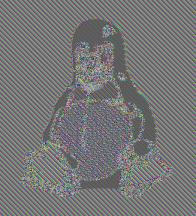
\includegraphics[width = 2 in]{pictures/duck-ecb.jpg}}
\hfill
\subfloat[Tryb CBC]{
\includegraphics[width = 2 in]{pictures/duck-cbc.jpg}}
\caption{Wpływ trybu CBC na wynik szyfrowania \cite{cbc-comparison}}
\label{fig:cbc-comparison}
\end{figure}

Aby zapobiec takim lukom w bezpieczeństwie stosowane są tryby wiązania bloków. W tym projekcie używany jest tryb CBC (ang. \textit{cipher block chaining}), który został wybrany ze względu na jego dużą popularność. Polega on na dodawaniu (operacja XOR) do bloków tekstu jawnego postaci zaszyfrowanych bloków poprzedzających (rys. \ref{fig:cbc}). W celu szyfrowania pierwszego bloku stosowany jest wektor inicjalizacji.

\begin{figure}[!h]
\centering
\subfloat[Szyfrowanie w trybie CBC]{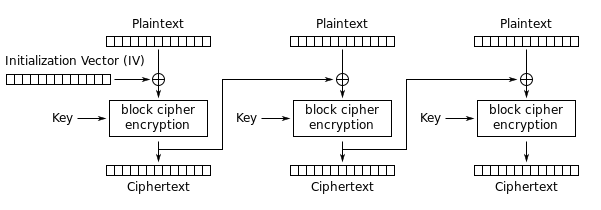
\includegraphics[width = \textwidth]{pictures/cbc-encryption.png}}
\newline
\subfloat[Deszyfrownaie w trybie CBC]{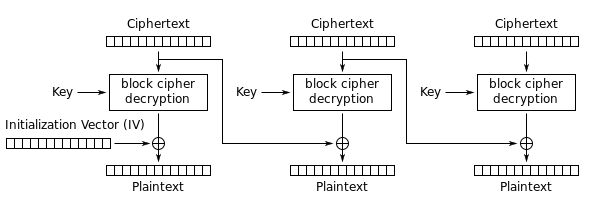
\includegraphics[width = \textwidth]{pictures/cbc-decryption.png}}
\caption{Sposób działania trybu wiązania bloków CBC \cite{cbc}}
\label{fig:cbc}
\end{figure}

Wiązanie boków w trybie CBC jest realizowane przez moduł \textit{communicator} (rozdz. \ref{sec:comminicator}). Operacja zaimplementowana jest przy pomocy bramek XOR:
\begin{itemize}
\item W przypadku szyfrowania bramka sumuje sygnał bloku do zaszyfrowania z zaszyfrowaną postacią bloku poprzedniego (lub wektorem inicjalizacji dla bloku pierwszego). Sygnał wyjściowy bramki połączony jest bezpośrednio do wejścia \textit{plaintext} modułu \textit{aes256enc} (rys. \ref{fig:communicator-schemat}).
\item W przypadku deszyfrowania bramka sumuje sygnał wyjściowy \textit{plaintext} modułu \textit{aes256dec} z zaszyfrowaną postacią bloku poprzedniego (lub wektorem inicjalizacji w przypadku bloku pierwszego). Sygnał wyjściowy bramki interpretowany jest jako postać jawna bloku (rys. \ref{fig:communicator-schemat}).
\end{itemize}